% !TeX program = lualatex
% !TeX encoding = UTF-8
% !TeX spellcheck = en_US
% !BIB program = biber
%% 
%% The above lines help editors like TeXstudio to automatically choose the right tools
%% to compile your LaTeX source file. If your tool does not support these magic comments,
%% you will need to make appropriate manual choices.
%% 
%% You can safely use "pdflatex" instead of "xelatex" if you prefer the pdfLaTeX toolchain.
%% However, pdfLaTeX will not be able to deliver the professional font experience that you
%% will get with XeLaTeX. You can also safely use "lualatex" instead of "xelatex" while
%% preserving the professional font experience if you prefer the LuaLaTeX toolchain.
%% 
%% _Important_: These magic comments should be on the first lines of your source file.
%% 
%%%%%%%%%%%%%%%%%%%%%%%%%%%%%%%%%%%%%%%%%%%%%%%%%%%%%%%%%%%%%%%%%%%%%%%%%%%%%%%%

%%%%%%%%%%%%%%%%%%%%%%%%%%%%%%%%%%%%%%%%%%%%%%%%%%%%%%%%%%%%%%%%%%%%%%%%%%%%%%%%
%% 
%%            JJJJ   K                         K   UUUU         UUUU  
%%            JJJJ   KKKK                   KKKK   UUUU         UUUU  
%%            JJJJ   KKKKKK               KKKKKK   UUUU         UUUU  
%%            JJJJ      KKKKKK         KKKKKK      UUUU         UUUU  
%%            JJJJ         KKKKKK   KKKKKK         UUUU         UUUU  
%%            JJJJ            KKKKKKKKK            UUUU         UUUU  
%%    JJ     JJJJJ               KKK               UUUUU       UUUUU  
%%  JJJJJJJJJJJJJ    KKKKKKKKKKKKKKKKKKKKKKKKKKK    UUUUUUUUUUUUUUU   
%%    JJJJJJJJJ      KKKKKKKKKKKKKKKKKKKKKKKKKKK      UUUUUUUUUUU     
%% 
%% This is an example file for using the JKU LaTeX technical report template
%% for your technical report.
%% 
%% Template created by Michael Roland (2021)
%% 
%%%%%%%%%%%%%%%%%%%%%%%%%%%%%%%%%%%%%%%%%%%%%%%%%%%%%%%%%%%%%%%%%%%%%%%%%%%%%%%%

%%%%%%%%%%%%%%%%%%%%%%%%%%%%%%%%%%%%%%%%%%%%%%%%%%%%%%%%%%%%%%%%%%%%%%%%%%%%%%%%
%% 
%% Document class: This is a koma-script article.
%% 
\documentclass[a4paper,oneside,10pt,ngerman,english]{scrartcl}
%% 
%% The comma-separated list in square brackets are class options.
%% Useful options that you might want to use:
%% 
%% Paper size:
%%  * a4paper ... A4 paper size
%% 
%% Optimize for single-sided or double-sided printing:
%%  * oneside ... single-sided
%%  * twoside ... double-sided
%% 
%% Base font size:
%%  * 10pt ... 10-pt font is used for normal text
%%  * 11pt ... 11-pt font is used for normal text
%% 
%% Define document languages (the last specified language becomes the document default
%% language):
%%  * ngerman ... German
%%  * english ... English
%%  * ...
%% 
%% Alternate document classes: The JKU report template supports the koma-script classes
%% `scrartcl', `scrreprt' and `scrbook'. The article class `scrartcl' is well-suited
%% for a typical technical report. However, `scrbook' or `scrreprt' may be better
%% suited for longer reports since they permit structuring your work in chapters.
%%  
%% _Important_: The document class should be the first line of LaTeX code in your main
%% source file. Do not place anything but comments / magic comments above that line (unless
%% you really know what you are doing).
%% 
%%%%%%%%%%%%%%%%%%%%%%%%%%%%%%%%%%%%%%%%%%%%%%%%%%%%%%%%%%%%%%%%%%%%%%%%%%%%%%%%

%%%%%%%%%%%%%%%%%%%%%%%%%%%%%%%%%%%%%%%%%%%%%%%%%%%%%%%%%%%%%%%%%%%%%%%%%%%%%%%%
%% 
%% Treat input files as UTF-8 encoded. Make sure to always load this when you use pdfLaTeX
%% so that pdfLaTeX knows how to read and interpret characters in this source file.
%% 
\usepackage[utf8]{inputenc}
%% 
%%%%%%%%%%%%%%%%%%%%%%%%%%%%%%%%%%%%%%%%%%%%%%%%%%%%%%%%%%%%%%%%%%%%%%%%%%%%%%%%

%%%%%%%%%%%%%%%%%%%%%%%%%%%%%%%%%%%%%%%%%%%%%%%%%%%%%%%%%%%%%%%%%%%%%%%%%%%%%%%%
%% 
%% Use the JKU LaTeX technical report template for this document.
%% 
\usepackage[techreport,fancyfonts,noautopdfinfo]{jkureport}
%% 
%% The comma-separated list in square brackets are theme options. Useful options that you
%% might want to use:
%% 
%% Document type:
%%  * phdthesis     ... PhD thesis.
%%  * mathesis      ... Master's thesis.
%%  * diplomathesis ... Diploma thesis.
%%  * bathesis      ... Bachelor's thesis.
%%  * seminarreport ... Seminar report.
%%  * techreport    ... Technical report.
%% 
%% Color scheme selection options:
%%  * JKU  ... Use JKU (gray) color scheme (this is the default if no scheme is selected).
%%  * BUS  ... Use Business School color scheme.
%%  * LIT  ... Use Linz Institute of Technology color scheme.
%%  * MED  ... Use MED faculty color scheme.
%%  * RE   ... Use RE faculty color scheme.
%%  * SOE  ... Use School of Education color scheme.
%%  * SOWI ... Use SOWI faculty color scheme.
%%  * TNF  ... Use TNF faculty color scheme.
%% 
%% Space-efficient monospace font options (requires XeTeX/LuaTeX):
%%  * compactmono   ... Use condensed fixed-width font everywhere.
%%  * nocompactverb ... Do not use condensed fixed-width font for verbatim and listings.
%% 
%% Style-breaking options:
%%  * noimprint      ... Do not insert imprint on title pages.
%%  * nojkulogo      ... Do not insert JKU & K logos on title pages.
%%  * capstitle      ... Set document title in capital letters.
%%  * nofancyfonts   ... Do not use custom TTF fonts with XeTeX/LuaTeX / supress pdfLaTeX warning.
%%  * equalmargins   ... Decrease the outer page margin to have both page margins of equal size
%%                       (the additional outer margin is intentional and to be used for
%%                       anotations; equalmargins also causes the text width to be
%%                       significantly larger than optimal for reading).
%% 
%% Experimental options:
%%  * mathastext ... Use standard document fonts (enhanced with symbols from Fira Math font
%%                   when using XeTeX/LuaTeX) in math mode.
%% 
%% Advanced options:
%%  * noautopdfinfo     ... Do not automatically try to add pdfinfo with hyperref from document
%%                          metadata fields.
%%  * logopath={<path>} ... Set the path where the theme can find its own logo resources. This
%%                          should typically be a relative path and the default is `./logos'.
%%  * fontpath={<path>} ... Set the path where the theme can find its own font resources. This
%%                          should typically be a relative path and the default is `./fonts'.
%% 
%% Hint: Boolean options can be used in the forms `option' or `option=true' the enable the
%% option and `nooption' or `option=false' to disable the option.
%% 
%%%%%%%%%%%%%%%%%%%%%%%%%%%%%%%%%%%%%%%%%%%%%%%%%%%%%%%%%%%%%%%%%%%%%%%%%%%%%%%%

%%%%%%%%%%%%%%%%%%%%%%%%%%%%%%%%%%%%%%%%%%%%%%%%%%%%%%%%%%%%%%%%%%%%%%%%%%%%%%%%
%% 
%% This is the place where you can load additional packages. If you want to load
%% a package `biblatex', you would use the command `\usepackage{biblatex}'.
%% 

\usepackage{csquotes}
\usepackage[backend=biber,citestyle=numeric,sortcites=true,maxcitenames=2,style=ACM-Reference-Format]{biblatex}
\setcounter{biburlnumpenalty}{100} %% reducing biburl* penalties typically improves URL placement in bibliography
\setcounter{biburllcpenalty}{100}
\setcounter{biburlucpenalty}{100}
\usepackage{todonotes}
\usepackage{import}
\usepackage{amsfonts}
\usepackage{subcaption}
\usepackage{float}
\usepackage{tikz}
\usepackage{pgfplots}
\pgfplotsset{compat=1.18}
\usepgfplotslibrary{statistics}
\usepackage{pgfplotstable}
\usepackage{minted}
\usepackage{booktabs}
\usetikzlibrary{fit,shapes,arrows,positioning,patterns}
%\usepackage{acronym}

%% 
%%%%%%%%%%%%%%%%%%%%%%%%%%%%%%%%%%%%%%%%%%%%%%%%%%%%%%%%%%%%%%%%%%%%%%%%%%%%%%%%

%%%%%%%%%%%%%%%%%%%%%%%%%%%%%%%%%%%%%%%%%%%%%%%%%%%%%%%%%%%%%%%%%%%%%%%%%%%%%%%%
%% 
%% Bibliography data files.
%% 

\addbibresource{references.bib}

%% 
%%%%%%%%%%%%%%%%%%%%%%%%%%%%%%%%%%%%%%%%%%%%%%%%%%%%%%%%%%%%%%%%%%%%%%%%%%%%%%%%

\begin{document}
%%%%%%%%%%%%%%%%%%%%%%%%%%%%%%%%%%%%%%%%%%%%%%%%%%%%%%%%%%%%%%%%%%%%%%%%%%%%%%%%
%% 
%% Report information and title page
%% 

%% Command \title{title}: sets the title of your report
\title{Analysis of Power Consumption of Home and SME Network Devices}

%% Set PDF metadata for standards compliance
\hypersetup{
    pdftitle={Analysis of Power Consumption of Home and SME Network Devices},
    pdfauthor={Michael Reinegger},
    pdfsubject={Technical Report - Master Project},
    pdfkeywords={Power Consumption, Network Devices, Home Router, SME Equipment, Energy Efficiency}
}

%% Command \titleshort{short title}: sets an abbreviated version of the report title for page heads
%\titleshort{Optional space for your abbreviated title}

%% Command \subtitle{subtitle}: sets the subtitle for seminar/technical reports (not used for theses)
\subtitle{Technical Report\\%
    \usekomafont{subtitlesmall}%
    \hfill\\%
    Master Project about the Analysis of Power Consumption of different Home and SME Network Equipment.
    \hfill\\%
}

%% Command \author{name}: sets the author name(s); separate multiple authors with \and; use \prefix{}
%%   and \suffix{} to add academic titles and suffixes (if needed); use \affiliation{} to add an
%%   affiliation, use \authornewline to add line breaks (e.g. to separate authors from contact
%%   information), use \authormail{}, \authorweb{}, \authorphone{} and \authorfax{} to add contact
%%   information)
\author{%
    Michael Reinegger
    \affiliation{Institute of Networks~and~Security}
    \authornewline
    \authormail{k12102754@students.jku.at}
    \authornewline
}

%% Command \date{YYYY-MM-DD}: set the day of publication (defaults to today)
%\date{2020-04-09}

%% Command \partnerlogo{filename}: use filename as partnerlogo, filename may be blank to disable the logo
%\partnerlogo{logos/ins}

%% Command \revisionblock{text}: set the document revision block on the title page
\revisionblock{V0.1 Initial Topic definition + Research Questions + Initial Test Setup and potential future Setup Ideas}

%% Command \reportnumber{number}: set the report number
%\reportnumber{Space for your report number}

%% Command \setbottommark{text}: set the bottom mark (in document footer)
%\setbottommark{Space for your bottom mark}

%% Command \abstract{text}: set the document abstract on the title page
%%\abstract{Space for your (short) abstract.}

%% Command \keywords{text}: set the document keywords
%\keywords{Space for your comma-separated keywords}


%% Finally, print the title page using the above information:
\maketitle
%% 
%%%%%%%%%%%%%%%%%%%%%%%%%%%%%%%%%%%%%%%%%%%%%%%%%%%%%%%%%%%%%%%%%%%%%%%%%%%%%%%%

%%%%%%%%%%%%%%%%%%%%%%%%%%%%%%%%%%%%%%%%%%%%%%%%%%%%%%%%%%%%%%%%%%%%%%%%%%%%%%%%
%% 
%% Add a table of contents
%% 

%% Make sure to start the table of contents on a new odd page (odd is only relevant in twoside layout)
\cleardoubleoddpage
%% Print the table of contents
\setcounter{secnumdepth}{3}
\setcounter{tocdepth}{2}  % Show up to subsections in TOC (section=1, subsection=2, subsubsection=3)
\tableofcontents

%% Make sure to start the list of acronyms on a new odd page (odd is only relevant in twoside layout)
%\cleardoubleoddpage
%% Include list of acronyms (optional and often not necessary)
%\import{./}{acronyms}

%% 
%%%%%%%%%%%%%%%%%%%%%%%%%%%%%%%%%%%%%%%%%%%%%%%%%%%%%%%%%%%%%%%%%%%%%%%%%%%%%%%%

%%%%%%%%%%%%%%%%%%%%%%%%%%%%%%%%%%%%%%%%%%%%%%%%%%%%%%%%%%%%%%%%%%%%%%%%%%%%%%%%
%% 
%% Abstract: Instead of an abstract on the title page (see \abstract{...}), you
%% sometimes want to add an abstract as its own unnumbered section.
%% 

%% (Optionally) let the abstract start on a new odd page (odd is only relevant in twoside layout)
\cleardoubleoddpage

\addsec{Abstract}
\todo{Rewrite abstract in formal academic style. Add: (1) motivation with EU/global energy stats for always-on networking equipment, (2) mention the custom Go-based measurement webapp, (3) summarize key quantitative findings (e.g., idle power ranges, load deltas), (4) state significance / practical recommendations.}
This project provides a comprehensive analysis of the power consumption of network devices in home and Small and Medium-sized Enterprise (SME) environments. We investigate how factors such as network load, the number of connected clients, and connection types (Ethernet vs. Wi-Fi) influence energy usage. Using a dedicated testbed with automated data collection, we evaluate the real-world power efficiency of various consumer-grade, ISP-provided, and business-grade devices. The findings can lead to reducing energy consumption with more energy-efficient network devices and configurations.

%% 
%%%%%%%%%%%%%%%%%%%%%%%%%%%%%%%%%%%%%%%%%%%%%%%%%%%%%%%%%%%%%%%%%%%%%%%%%%%%%%%%

%%%%%%%%%%%%%%%%%%%%%%%%%%%%%%%%%%%%%%%%%%%%%%%%%%%%%%%%%%%%%%%%%%%%%%%%%%%%%%%%
%% 
%% Add your report sections ...
%% 

%% (Optionally) let the main sections start on a new odd page (odd is only relevant in twoside layout)
\cleardoubleoddpage

\section{Introduction}
\label{sec:introduction}
\todo{Polish introduction prose. Add: opening paragraph with global energy context (cite IEA/EU stats on ICT energy), narrow down to home/SME CPE devices specifically, clearly state the gap (lack of independent, reproducible measurements), state contribution (custom automated test framework + systematic multi-device analysis), brief outline of report structure.}

This project aims to analyze the power consumption of various network devices commonly used in home and small-to-medium enterprise (SME) environments. The equipment under investigation ranges from consumer-grade home routers to ISP-provided devices and business-grade switches and access points. The goal is to create a comprehensive overview of power consumption across different scenarios and usage patterns.

The analysis will examine several factors that influence power consumption: the number of active Ethernet ports, the number of connected Wi-Fi clients, varying levels of network load and so on. Data will be collected using a smart power meter capable of providing time-based power consumption measurements. This meter is integrated with a monitoring stack (Prometheus and Grafana) to enable automated data collection and visualization.

With this data, we can evaluate the efficiency of these devices under different conditions and identify which configurations are most power-efficient for specific use cases. For example, we can compare whether using an ISP-provided router in bridge mode is more efficient than using a separate router and switch/modem combination. Additionally, the analysis will help determine if some devices should be powered down during periods of low activity, such as overnight, to conserve energy.


\section{Research Questions}
\label{sec:research-questions}
\todo{Consider restructuring RQs into primary (RQ1--RQ3) and secondary (RQ4--RQ9) groups. Add a brief introductory paragraph explaining how these RQs were derived.}
The following research questions guide this investigation:
\begin{enumerate}
    \item[\textbf{RQ1}] How does power consumption change with the number of active Ethernet ports?
    \label{rq:ports}
    \item[\textbf{RQ2}] Is there a measurable difference between 100\,Mbps and 1\,Gbps connections, in different load scenarios?
    \label{rq:speed}
    \item[\textbf{RQ3}] How does power consumption scale with network load (idle, 50\%, 100\% utilization of bandwidth)?
    \label{rq:load-scaling}
    \item[\textbf{RQ4}] Which equipment is suitable for continuous operation and which devices have high idle consumption that makes them candidates for automated shutdown during off-peak hours?
    \label{rq:idle-suitability}
    \item[\textbf{RQ5}] How does power consumption per client differ between Ethernet and Wi-Fi connections? Is there a threshold where Wi-Fi becomes more efficient on a per-client basis?
    \label{rq:eth-vs-wifi}
    \item[\textbf{RQ6}] What is the actual impact of power-saving modes on overall power consumption?
    \label{rq:power-saving}
    \item[\textbf{RQ7}] Does the type of connected device (smartphone, laptop, IoT device) or the wireless signal strength (distance to access point) affect power consumption?
    \label{rq:device-type}
    \item[\textbf{RQ8}] Does a device's maximum power consumption rating correlate with its real-world power usage under typical operating conditions, and what does it take to reach that level?
    \label{rq:rated-vs-real}
    \item[\textbf{RQ9}] How efficient is ISP-provided equipment (e.g., Huawei router or Fritzbox 7530) when operating in bridge mode compared to dedicated networking equipment?
    \label{rq:bridge-mode}
    \todo{Decide whether to keep RQ9 or merge with RQ4.}
\end{enumerate}

\section{Setup}
\label{sec:setup}
    \subsection{Hardware}
    List of available network devices: (That I have lying around)
    \begin{description}
        \item[Fritzbox 7530] (2018, 802.11ac, 4$\times$ GbE, 18\,W max)
        \item[Asus RT-AX68U] (2020, 802.11ax, 4$\times$ GbE, 33\,W max)
        \item[Alcatel HH40V] (2018, 802.11n, 2$\times$ 100 Mbps, 10\,W max)
        \item[Huawei EchoLife EG8245W5-8T] (2020, 802.11ax, 4$\times$ GbE, 24\,W max)
    \end{description}
    \subsection{Sampling Rate and Accuracy of Power Meter}
    The exact sampling rate of the power meter is not specified in its documentation. However, for the purpose of this analysis, Prometheus is configured to sample data every 10 seconds, which should be sufficient for most tests. The power measurement accuracy is rated at $\pm 100$\,mW for readings below 5\,W and $\pm 2\%$ for readings above 5\,W.
   
    After some testing i found the sampe rate of the power meter to be around once every 2 minutes. This is quite slow and makes it hard to measure short load spikes for example.
    Because of that longer test phases are needed to get meaningful data.

    But i discovered that there exists a workaround to increase the polling rate of the power meter by using the a simple home assistant script that set the power meter to "on" every 15 seconds to get more frequent measurements.

    % code for home assistant script
    \begin{minted}{yaml}
        alias: Automation - Nudge FritzDECT Smart Plug
        description: ""
        triggers:
        - trigger: time_pattern
            seconds: /15
        conditions:
        - condition: state
            entity_id: switch.fritz_dect_200
            state: "on"
        - condition: time
            after: "06:30:00"
            before: "23:59:00"
        actions:
        - action: switch.turn_on
            target:
            entity_id: switch.fritz_dect_200
        mode: single
    \end{minted}

    \subsection{Initial Testing Setup}
    Initial testing setup, shown in figure \ref{fig:initial_network_layout}, uses the Fritzbox to connect to the Power Meter using DECT.
    Then the Fritzbox is connected to my home network such that I can reach the Fritzbox from my NanoPi Neo3.
        \begin{figure}[H]
            \centering
            \includegraphics[width=0.8\textwidth]{images/initial_network_layout.png}
            \caption{Initial Network Layout}
            \label{fig:initial_network_layout}
        \end{figure}

    One can already see, in Figure \ref{fig:grafana_power_consumption}, the larger power consumption when running \texttt{iperf} in the first third. Everywhere else the small spikes are something that happens periodically.
    However, I am not able to say what exactly causes these small spikes yet.

        \begin{figure}[H]
            \centering
            \includegraphics[width=0.8\textwidth]{images/grafana_power_consumption.png}
            \caption{Grafana Dashboard showing Fritzbox Power Consumption}
            \label{fig:grafana_power_consumption}
        \end{figure}

    Now the device to test can be connected to the power meter and the Fritzbox can collect the power consumption data.
    Also, the device to test can be connected to the home network and be put under load without interfering with the data collection.
    This was a problem as I initially wanted to test the FritzBox, that is connected to the power meter, itself but that caused data loss due to the API of the Fritzbox being unresponsive under load.

    \subsection{Potential future Setup Ideas}
    Since the FritzBox allows data collection of smart home devices via the TR064 API we can use e.g. gofritz https://github.com/nitram509/gofritz to create a script
    that collects the data while also being able to create load for the testing devices/automate scenarios and therefore create a fully automated testing setup that can also annotate
    the collected data with the current load situation (low load, high load, testing different amount of clients, LAN cables connected, etc.).
    Maybe even a Web UI where one can directly annotate the data for manual testing. Like click button to start and enter Text of test e.g. Connect 5 LAN cables. And then click stop to end the test and maybe also directly export the data and or screenshots of the graphs.

    \subsection{Automating Testing and Data Collection}
    \label{sec:automation}
    \todo{Polish prose into formal academic style throughout this subsection.}
    To enable reproducible, automated measurements, we developed a custom web application with a Go backend and a JavaScript frontend.
    The source code is available at \texttt{github.com/MrCodeEU/jku-master-project-network-devices-power-consumption-analysis}.

    \subsubsection{Architecture Overview}
    The application consists of several components:
    \begin{description}
        \item[Test Runner (\texttt{runner.go})] Orchestrates test execution in three phases: pre-test baseline, load test (with per-interface ramping), and post-test baseline. Each phase duration, interface activation order, and ramp steps are configurable via the web UI.
        \item[Load Generator (\texttt{loadgen.go})] Generates network traffic via UDP flooding, TCP connections, or raw Layer~2 Ethernet frames. Per-interface rate limiting is implemented using a spin-wait loop with nanosecond precision. The generator supports configurable packet sizes, worker counts per interface, and target throughput levels.
        \item[Power Meter Interface (\texttt{fritzbox.go})] Reads real-time power consumption from a FritzBox DECT~200 smart plug via the TR-064 SOAP API, using the \texttt{gofritz} library. A separate FritzBox (not the device under test) is used for data collection to avoid measurement interference.
        \item[Web Server (\texttt{server.go})] Exposes a REST API and serves the frontend. Real-time data streaming to the browser uses Server-Sent Events (SSE). Test results are persisted in an SQLite database with full configuration, time-series data, and computed per-phase statistics.
        \item[Analysis Dashboard (\texttt{analysis.js})] A client-side analysis page that loads test data from the database or imported CSV files. It computes per-phase statistics (average, standard deviation, min/max power and throughput, efficiency in Mbps/W) and renders interactive Chart.js visualizations. Export options include CSV, Excel, and pgfplots-compatible formats for direct use in \LaTeX\ reports.
    \end{description}

    \subsubsection{Load Generation Approach}
    \todo{Add a table comparing TCP vs UDP vs Layer~2 performance.}
    We evaluated three traffic generation methods:
    \begin{itemize}
        \item \textbf{TCP}: Largely rejected by devices under test; achieved only 60--80\,Mbps as most consumer routers drop or rate-limit unsolicited TCP connections to their management interface.
        \item \textbf{UDP flooding}: The primary method used. Achieves near line-rate throughput (e.g., 3.85\,Gbps aggregate on the Huawei EG8245W5-8T across 4$\times$1\,GbE ports). Uses 1400-byte packets with 16 workers per interface and batched sending (10 packets per sleep cycle).
        \item \textbf{Layer~2 raw frames}: Implemented via \texttt{libpcap} for direct Ethernet frame injection. On Windows, throughput was limited to approximately 550--600\,Mbps due to OS-level packet scheduling constraints.
    \end{itemize}
    UDP flooding was selected as the primary load generation method due to its ability to saturate gigabit links reliably across all tested devices.

    \subsubsection{Power Meter Polling Rate}
    The FritzBox DECT~200 smart plug natively updates its power reading only approximately once every two minutes, which is insufficient for capturing transient power behavior. To increase the effective polling rate, a Home Assistant automation was employed that sends a ``turn on'' command to the already-on smart plug every 15 seconds. This triggers the DECT~200 to refresh its power reading, achieving an effective polling interval of approximately 15 seconds. The test application then queries the updated value via TR-064 every 5 seconds.
    \todo{Add citation for TR-064 protocol specification and gofritz library.}

% ===========================================================================
% Section 4: Test Setups
% ===========================================================================
\section{Test Setups}
\label{sec:test-setups}

This section describes the test setups used to investigate the research questions defined in Section~\ref{sec:research-questions}.
Each test setup specifies the devices under test, physical topology, traffic generation method, and measurement protocol.
\todo{Add introductory paragraph linking test design philosophy (automated, reproducible, phased).}

% ---------------------------------------------------------------------------
\subsection{Test~1: Incremental Port Load Test (Completed)}
\label{sec:test-incremental-port-load}
% ---------------------------------------------------------------------------

This test investigates how power consumption changes as Ethernet ports are incrementally loaded with maximum UDP traffic.
It directly addresses \textbf{RQ1} (power vs.\ number of active ports) and provides partial data for \textbf{RQ4} (idle power suitability for continuous operation) and \textbf{RQ8} (rated vs.\ real-world maximum power).

\subsubsection{Devices Under Test}
Four devices were tested, representing a range of consumer and ISP-provided equipment:
\begin{description}
    \item[Fritzbox 7530] (2018, 802.11ac, 4$\times$ GbE LAN, rated 18\,W max)
    \item[Asus RT-AX68U] (2020, 802.11ax, 4$\times$ GbE LAN, rated 33\,W max)
    \item[Huawei EchoLife EG8245W5-8T] (2020, 802.11ax, 4$\times$ GbE LAN, rated 24\,W max)
    \item[Alcatel HH40V] (2018, 802.11n, 2$\times$ 100\,Mbps LAN, rated 10\,W max)
\end{description}

\subsubsection{Physical Topology}
Figure~\ref{fig:test1_topology} shows the physical test setup.
The PC (equipped with a 4-port 2.5\,GbE NIC) connects 1--4 Ethernet cables to the device under test (DUT), which is powered through the DECT~200 smart plug for power measurement.
A \emph{separate} Fritzbox~7530 (not under test) hosts the DECT~200 base station and provides the TR-064 API endpoint for reading power data.
This isolation is critical: under heavy CPU load, the DUT's management API becomes unresponsive, which would cause measurement gaps if the DUT itself were used for data collection.

\begin{figure}[H]
    \centering
    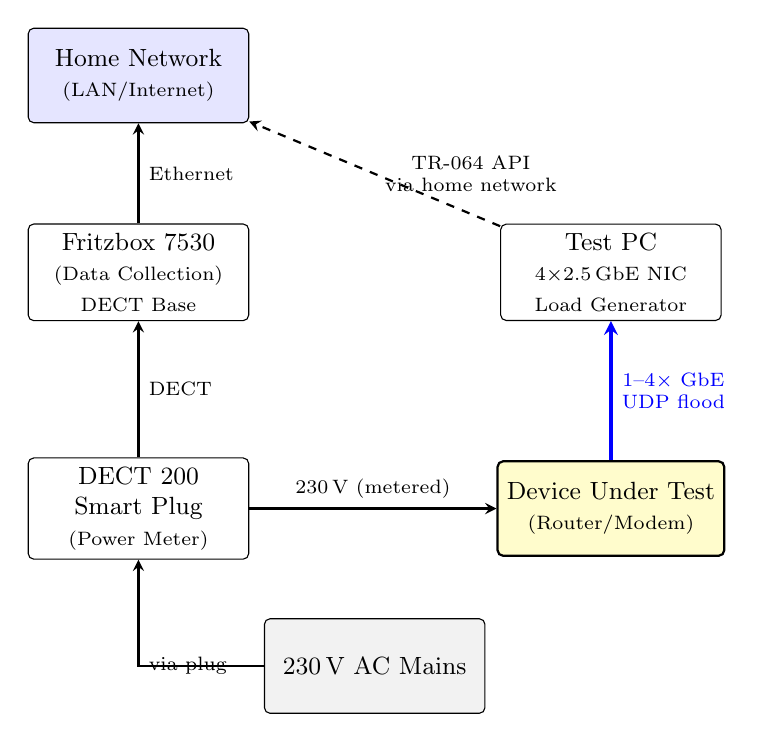
\begin{tikzpicture}[
        box/.style={rectangle, draw, minimum width=2.8cm, minimum height=1.2cm, text centered, font=\small, align=center, rounded corners=2pt},
        dut/.style={box, fill=yellow!20, thick},
        arrow/.style={->, >=stealth, thick},
        dashedarrow/.style={->, >=stealth, thick, dashed},
        lbl/.style={font=\scriptsize, midway, align=center}
    ]
        % Power Meter
        \node[box] (meter) at (0,0) {DECT~200\\Smart Plug\\{\scriptsize (Power Meter)}};

        % Data Collection Fritzbox
        \node[box] (fritzbox) at (0,3) {Fritzbox 7530\\{\scriptsize (Data Collection)}\\{\scriptsize DECT Base}};

        % Device Under Test
        \node[dut] (dut) at (6,0) {Device Under Test\\{\scriptsize (Router/Modem)}};

        % Main PC
        \node[box] (pc) at (6,3) {Test PC\\{\scriptsize 4$\times$2.5\,GbE NIC}\\{\scriptsize Load Generator}};

        % Home Network
        \node[box, fill=blue!10] (network) at (0,5.5) {Home Network\\{\scriptsize (LAN/Internet)}};

        % AC Power
        \node[box, fill=gray!10] (mains) at (3,-2) {230\,V AC Mains};

        % Connections
        \draw[arrow] (meter) -- node[right, lbl] {DECT} (fritzbox);
        \draw[arrow] (fritzbox) -- node[right, lbl] {Ethernet} (network);
        \draw[dashedarrow] (pc) -- node[right, lbl] {TR-064 API\\{\scriptsize via home network}} (network);
        \draw[arrow] (mains) -| node[near end, right, lbl] {via plug} (meter);
        \draw[arrow] (meter) -- node[above, lbl] {230\,V (metered)} (dut);
        \draw[arrow, very thick, blue] (dut) -- node[right, lbl, text=blue] {1--4$\times$ GbE \\{\scriptsize UDP flood}} (pc);

    \end{tikzpicture}
    \caption{Physical topology for the Incremental Port Load Test. The DUT is powered through the DECT~200 smart plug. A separate Fritzbox handles power data collection via DECT and TR-064.}
    \label{fig:test1_topology}
\end{figure}

\subsubsection{Test Protocol}
Each device was tested using the following automated protocol, executed by the custom web application described in Section~\ref{sec:automation}:
\begin{enumerate}
    \item \textbf{Pre-test baseline} (10\,min): All Ethernet cables connected but no traffic generated. Measures idle power with active link-up on all ports.
    \item \textbf{Load phase~1} (20\,min): Maximum UDP flood on \textbf{1~port} (target: 1\,Gbps).
    \item \textbf{Load phase~2} (20\,min): Maximum UDP flood on \textbf{2~ports} (target: 2\,Gbps).
    \item \textbf{Load phase~3} (20\,min): Maximum UDP flood on \textbf{3~ports} (target: 3\,Gbps). \emph{Skipped for Alcatel~HH40V (only 2 ports).}
    \item \textbf{Load phase~4} (20\,min): Maximum UDP flood on \textbf{4~ports} (target: 4\,Gbps). \emph{Skipped for Alcatel.}
    \item \textbf{Post-test baseline} (20\,min): All traffic stopped, cables remain connected. Measures power recovery behavior.
\end{enumerate}

\noindent\textbf{Load generation parameters:}
\begin{itemize}
    \item Protocol: UDP, packet size: 1400\,bytes, 16 workers per interface
    \item Target: device's own IP address (e.g., \texttt{169.254.1.1:80} for Fritzbox)
    \item Interfaces activated incrementally with 5 ramp-up steps per interface
    \item Power polling interval: 5\,seconds (via TR-064 SOAP API)
\end{itemize}

\noindent\textbf{Important limitation:} Traffic is directed at the DUT's own IP address, meaning all packets are processed by the device's \emph{CPU/software stack}, not merely switched at Layer~2 by the switching ASIC. This represents a CPU-intensive workload (similar to heavy NAT processing or connection handling) rather than pure L2 forwarding. As a result, devices with weaker CPUs (notably the Fritzbox~7530) show throughput degradation at higher port counts due to CPU saturation, not switching fabric limitations.

\subsubsection{Research Questions Addressed}
\begin{description}
    \item[RQ1 (Fully addressed):] The test directly measures power at 0, 1, 2, 3, and 4 active loaded ports, providing a complete port-count vs.\ power profile for each device.
    \item[RQ4 (Partially addressed):] The 10-minute pre-test baseline provides idle power measurements (with cables connected) for all four devices, enabling an idle power comparison and annual energy cost estimation. A full 24-hour idle measurement is not captured.
    \item[RQ8 (Partially addressed):] By comparing the maximum observed power under full Ethernet load to the manufacturer's rated maximum, we can assess how close real-world usage comes to the rated specification. This test does not activate Wi-Fi or USB peripherals, so the absolute maximum is not reached.
\end{description}

% ---------------------------------------------------------------------------
\subsection{Test~2: Throughput Scaling and Link Speed (Planned)}
\label{sec:test-throughput-scaling}
% ---------------------------------------------------------------------------

This test combines two research questions into a single measurement campaign by varying both throughput level and link speed on a single Ethernet port.
It directly addresses \textbf{RQ2} (100\,Mbps vs.\ 1\,Gbps) and \textbf{RQ3} (power vs.\ throughput at intermediate load levels).

\subsubsection{Devices Under Test}
All four devices from Test~1. The Alcatel~HH40V (100\,Mbps ports) participates only in Run~B.

\subsubsection{Physical Topology}
The physical topology is identical to Test~1 (Figure~\ref{fig:test1_topology}): single Ethernet cable from test PC to DUT, power measured via DECT~200.
Figure~\ref{fig:test2_ramp_profile} shows the expected throughput profile for the ramp-step load generation.

\begin{figure}[H]
    \centering
    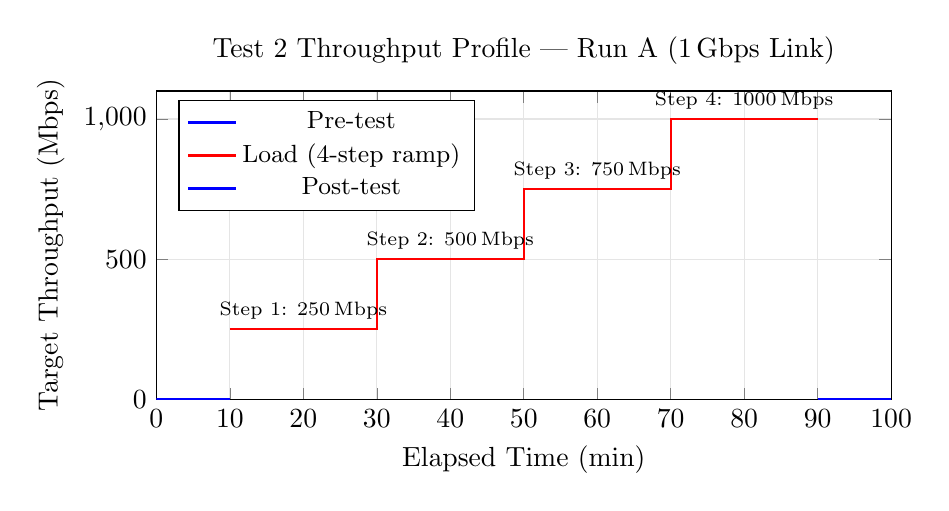
\begin{tikzpicture}
        \begin{axis}[
            width=0.90\linewidth,
            height=5.5cm,
            xlabel={Elapsed Time (min)},
            ylabel={Target Throughput (Mbps)},
            xmin=0, xmax=100,
            ymin=0, ymax=1100,
            grid=major,
            grid style={gray!20},
            title={Test~2 Throughput Profile --- Run~A (1\,Gbps Link)},
            legend pos=north west,
            legend style={font=\small},
        ]
            % Pre-test
            \addplot[blue, thick] coordinates {(0,0) (10,0)};
            \addlegendentry{Pre-test}
            % Ramp steps
            \addplot[red, thick] coordinates {(10,250) (30,250) (30,500) (50,500) (50,750) (70,750) (70,1000) (90,1000)};
            \addlegendentry{Load (4-step ramp)}
            % Post-test
            \addplot[blue, thick] coordinates {(90,0) (100,0)};
            \addlegendentry{Post-test}
            
            % Annotations
            \node[font=\scriptsize, anchor=south] at (axis cs:20,250) {Step 1: 250\,Mbps};
            \node[font=\scriptsize, anchor=south] at (axis cs:40,500) {Step 2: 500\,Mbps};
            \node[font=\scriptsize, anchor=south] at (axis cs:60,750) {Step 3: 750\,Mbps};
            \node[font=\scriptsize, anchor=south] at (axis cs:80,1000) {Step 4: 1000\,Mbps};
        \end{axis}
    \end{tikzpicture}
    \caption{Expected throughput profile for Test~2 Run~A. The load generator's ramp-step feature automatically transitions through four equal-duration steps. Run~B uses the same structure with 100\,Mbps maximum (steps at 25, 50, 75, 100\,Mbps).}
    \label{fig:test2_ramp_profile}
\end{figure}

\subsubsection{Test Protocol}
The test uses the load generator's built-in \emph{ramp steps} feature, which linearly increases the per-interface rate limit in equal increments.
Two runs are performed per device:

\paragraph{Run~A --- 1\,Gbps Link:}
\begin{enumerate}
    \item \textbf{Pre-test baseline} (10\,min): 1 cable connected, no traffic.
    \item \textbf{Load phase} (80\,min total): Single port, UDP, \texttt{ramp\_steps=4}, \texttt{target\_mbps=1000}.
    The load generator automatically steps through:
    \begin{itemize}
        \item Step~1 (20\,min): $\sim$250\,Mbps (25\% of link capacity)
        \item Step~2 (20\,min): $\sim$500\,Mbps (50\%)
        \item Step~3 (20\,min): $\sim$750\,Mbps (75\%)
        \item Step~4 (20\,min): $\sim$1000\,Mbps (100\%)
    \end{itemize}
    \item \textbf{Post-test baseline} (10\,min): Traffic stopped, cable remains connected.
\end{enumerate}

\paragraph{Run~B --- 100\,Mbps Link:}
Before starting, force the test PC's NIC to 100\,Mbps using Windows Device Manager or PowerShell:
\begin{verbatim}
    # PowerShell (run as Administrator):
    Set-NetAdapterAdvancedProperty -Name "Ethernet" `
        -DisplayName "Speed & Duplex" -DisplayValue "100 Mbps Full Duplex"
\end{verbatim}
Alternatively, use Device Manager $\rightarrow$ Network Adapters $\rightarrow$ Properties $\rightarrow$ Advanced $\rightarrow$ Speed \& Duplex $\rightarrow$ select \texttt{100 Mbps Full Duplex}.
Then repeat the same structure with \texttt{target\_mbps=100} and \texttt{ramp\_steps=4}, yielding steps at 25, 50, 75, and 100\,Mbps.
After completion, restore to auto-negotiation (typically 2.5\,Gbps on the Realtek controller):
\begin{verbatim}
    Set-NetAdapterAdvancedProperty -Name "Ethernet" `
        -DisplayName "Speed & Duplex" -DisplayValue "Auto Negotiation"
\end{verbatim}

\noindent\textbf{Load generation parameters (both runs):}
\begin{itemize}
    \item Protocol: UDP, packet size: 1400\,bytes, 16 workers
    \item Single interface enabled, \texttt{ramp\_duration} = 0 (auto, equals test duration)
    \item Target: DUT's own IP address (consistent with Test~1)
    \item Power polling interval: 5\,seconds
\end{itemize}

\subsubsection{Research Questions Addressed}
\begin{description}
    \item[RQ2 (Fully addressed):] Comparing idle power and power at matched throughput levels (e.g., 100\,Mbps via a 1\,GbE link vs.\ 100\,Mbps via a 100\,Mbps link) isolates the PHY-level power cost of the higher link speed.
    \item[RQ3 (Fully addressed):] The four-step ramp produces a power-vs-throughput curve at 25\%, 50\%, 75\%, and 100\% utilization for each link speed, revealing whether power scales linearly, sub-linearly, or in discrete steps.
\end{description}
\todo{Run this test and fill in results.}

% ---------------------------------------------------------------------------
\subsection{Test~3: Energy Efficiency and Extended Idle (Planned)}
\label{sec:test-energy-efficiency}
% ---------------------------------------------------------------------------

This test combines extended idle measurements with Energy-Efficient Ethernet (EEE, IEEE~802.3az) toggling to investigate both continuous-operation suitability and the real-world impact of power-saving features.
It directly addresses \textbf{RQ4} (idle power suitability) and \textbf{RQ6} (power-saving mode impact).

\subsubsection{Devices Under Test}
All four devices. EEE support will be verified per-device via \texttt{ethtool --show-eee} on connected ports.
Devices that do not support EEE will only undergo the extended idle portion.

\subsubsection{Physical Topology}
The physical topology is identical to Test~1 (Figure~\ref{fig:test1_topology}).
Figure~\ref{fig:test3_configurations} illustrates the three configuration variants.

\begin{figure}[H]
    \centering
    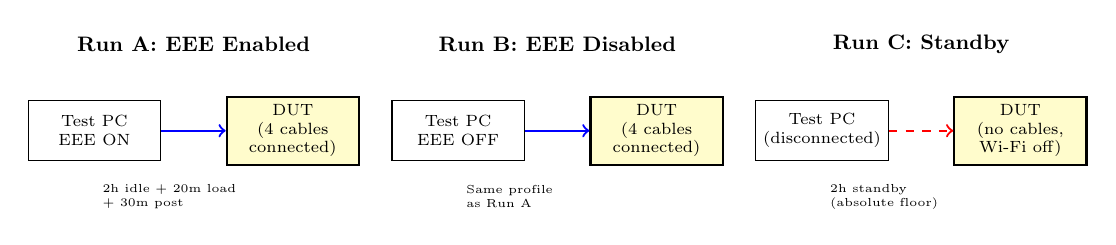
\begin{tikzpicture}[scale=0.84, transform shape,
        box/.style={rectangle, draw, minimum width=2.0cm, minimum height=0.9cm, text centered, font=\scriptsize, align=center},
        dut/.style={box, fill=yellow!20, thick},
        cable/.style={->, thick, blue},
        nocable/.style={->, thick, red, dashed},
    ]
        % Run A - EEE Enabled
        \node[font=\small\bfseries] at (0, 1.8) {Run A: EEE Enabled};
        \node[box] (pca) at (-1.5, 0.5) {Test PC\\EEE ON};
        \node[dut] (duta) at (1.5, 0.5) {DUT\\(4 cables\\connected)};
        \draw[cable] (pca) -- (duta);
        \node[font=\tiny, align=left, anchor=west] at (-1.5, -0.5) {2h idle + 20m load\\+ 30m post};
        
        % Run B - EEE Disabled
        \node[font=\small\bfseries] at (5.5, 1.8) {Run B: EEE Disabled};
        \node[box] (pcb) at (4, 0.5) {Test PC\\EEE OFF};
        \node[dut] (dutb) at (7, 0.5) {DUT\\(4 cables\\connected)};
        \draw[cable] (pcb) -- (dutb);
        \node[font=\tiny, align=left, anchor=west] at (4, -0.5) {Same profile\\as Run A};
        
        % Run C - No Cables
        \node[font=\small\bfseries] at (11, 1.8) {Run C: Standby};
        \node[box] (pcc) at (9.5, 0.5) {Test PC\\(disconnected)};
        \node[dut] (dutc) at (12.5, 0.5) {DUT\\(no cables,\\Wi-Fi off)};
        \draw[nocable] (pcc) -- (dutc);
        \node[font=\tiny, align=left, anchor=west] at (9.5, -0.5) {2h standby\\(absolute floor)};
    \end{tikzpicture}
    \caption{Test~3 configuration variants. Run~A and Run~B use the same physical setup but differ in EEE settings. Run~C disconnects all cables to measure true standby power.}
    \label{fig:test3_configurations}
\end{figure}

\subsubsection{Test Protocol}
Three runs are performed per device, requiring manual reconfiguration between runs:

\paragraph{Run~A --- EEE Enabled (Default):}
\begin{enumerate}
    \item Verify EEE is active: \texttt{ethtool --show-eee ethX} on the test PC.
    \item \textbf{Extended idle baseline} (2\,hours): All 4 cables connected, no traffic. Captures periodic background activity (DHCP renewal, Wi-Fi beaconing, firmware checks).
    \item \textbf{Load phase} (20\,min): 1 port, maximum UDP. Establishes a loaded power reference with EEE active.
    \item \textbf{Post-test recovery} (30\,min): Observe how quickly the device returns to idle power.
\end{enumerate}

\paragraph{Run~B --- EEE Disabled:}
\begin{enumerate}
    \item Disable EEE on test PC: \texttt{ethtool --set-eee ethX eee off}.
    \item If DUT exposes EEE settings (e.g., via admin UI), disable there as well.
    \item Repeat the same profile as Run~A (2\,h idle + 20\,min load + 30\,min post).
\end{enumerate}

\paragraph{Run~C --- Minimal Configuration (No Cables):}
\begin{enumerate}
    \item Disconnect all Ethernet cables from the DUT.
    \item Disable Wi-Fi via the DUT's admin interface (if possible).
    \item \textbf{Standby measurement} (2\,hours): Measures true standby power with no active interfaces.
\end{enumerate}

\noindent\textbf{Load generation parameters (Runs~A and B, load phase only):}
\begin{itemize}
    \item Protocol: UDP, packet size: 1400\,bytes, 16 workers, single interface
    \item \texttt{target\_mbps} = 0 (unlimited), no ramp steps
    \item Power polling interval: 5\,seconds
\end{itemize}

\subsubsection{Research Questions Addressed}
\begin{description}
    \item[RQ4 (Fully addressed):] The 2-hour idle measurements (with cables, without cables) provide a robust idle power characterization including any periodic background power fluctuations. Combined with the 10-minute baselines from Test~1, this enables confident annual energy cost projections and automated-shutdown recommendations.
    \item[RQ6 (Fully addressed):] Direct comparison of Run~A (EEE on) vs.\ Run~B (EEE off) at both idle and loaded states quantifies the real-world power savings from IEEE~802.3az. Run~C establishes the absolute floor.
\end{description}
\todo{Run this test and fill in results.}

% ---------------------------------------------------------------------------
\subsection{Test~4: Wi-Fi Impact and Maximum Load (Planned)}
\label{sec:test-wifi}
% ---------------------------------------------------------------------------

This test investigates the power cost of Wi-Fi by comparing Ethernet-only and Wi-Fi traffic paths, varying Wi-Fi band and distance, and finally combining all subsystems to approach the rated maximum power.
It addresses \textbf{RQ5} (Ethernet vs.\ Wi-Fi), \textbf{RQ7} (device type and signal strength), and completes \textbf{RQ8} (reaching rated maximum power).

\subsubsection{Devices Under Test}
Three devices with Wi-Fi: Fritzbox~7530 (802.11ac), Asus~RT-AX68U (802.11ax), Huawei~EG8245W5-8T (802.11ax).
The Alcatel~HH40V (802.11n, 2.4\,GHz only) may be included for a limited subset.

\subsubsection{Physical Topology}
Figure~\ref{fig:test4_wifi_topology} shows the physical setup for Runs~A--D (Wi-Fi traffic) and Run~E (combined Ethernet + Wi-Fi maximum load).

\begin{figure}[H]
    \centering
    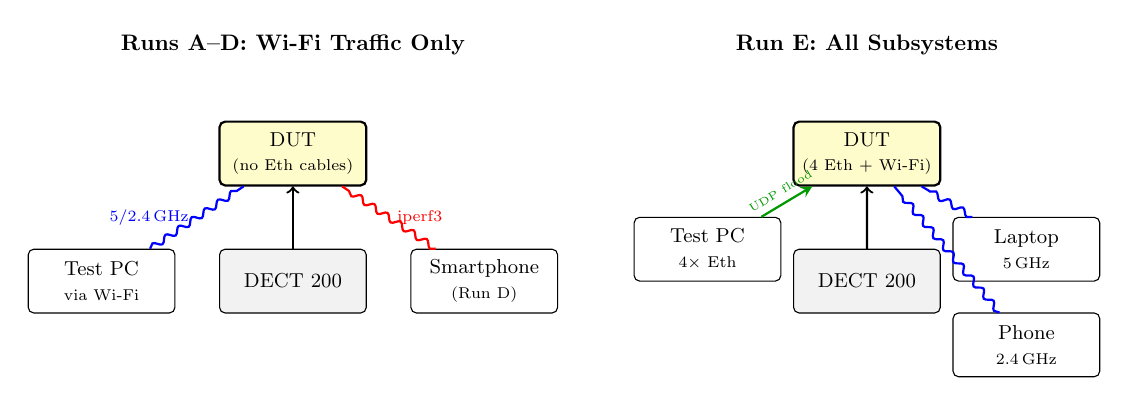
\begin{tikzpicture}[scale=0.81, transform shape,
        box/.style={rectangle, draw, minimum width=2.3cm, minimum height=1.0cm, text centered, font=\small, align=center, rounded corners=2pt},
        dut/.style={box, fill=yellow!20, thick},
        wifi/.style={decorate, decoration={snake, amplitude=0.4mm, segment length=2mm, post length=1mm}, thick, blue},
        eth/.style={->, >=stealth, thick, green!60!black},
    ]
        % Runs A-D: WiFi only
        \node[font=\bfseries] at (0, 4.2) {Runs A--D: Wi-Fi Traffic Only};
        \node[dut] (dut1) at (0, 2.5) {DUT\\{\scriptsize (no Eth cables)}};
        \node[box] (pc1) at (-3, 0.5) {Test PC\\{\scriptsize via Wi-Fi}};
        \node[box] (phone1) at (3, 0.5) {Smartphone\\{\scriptsize (Run D)}};
        \draw[wifi] (pc1) -- node[left, font=\scriptsize, midway] {5/2.4\,GHz} (dut1);
        \draw[wifi, red] (phone1) -- node[right, font=\scriptsize, midway] {iperf3} (dut1);
        \node[box, fill=gray!10] (meter1) at (0, 0.5) {DECT~200};
        \draw[->, thick] (meter1) -- (dut1);
        
        % Run E: Combined maximum
        \node[font=\bfseries] at (9, 4.2) {Run E: All Subsystems};
        \node[dut] (dut2) at (9, 2.5) {DUT\\{\scriptsize (4 Eth + Wi-Fi)}};
        \node[box] (pc2) at (6.5, 1) {Test PC\\{\scriptsize 4$\times$ Eth}};
        \node[box] (laptop2) at (11.5, 1) {Laptop\\{\scriptsize 5\,GHz}};
        \node[box] (phone2) at (11.5, -0.5) {Phone\\{\scriptsize 2.4\,GHz}};
        \draw[eth] (pc2) -- node[above, font=\tiny, sloped] {UDP flood} (dut2);
        \draw[wifi] (laptop2) -- (dut2);
        \draw[wifi] (phone2) -- (dut2);
        \node[box, fill=gray!10] (meter2) at (9, 0.5) {DECT~200};
        \draw[->, thick] (meter2) -- (dut2);
    \end{tikzpicture}
    \caption{Test~4 physical topologies. Runs~A--D use Wi-Fi-only traffic to isolate Wi-Fi power consumption. Run~E combines maximum Ethernet load (4 ports) with multiple Wi-Fi clients to approach the rated maximum power.}
    \label{fig:test4_wifi_topology}
\end{figure}

\subsubsection{Test Protocol}
Five runs are performed per device. Runs~A--D each follow the same structure: 10\,min idle, 20\,min load, 10\,min post.
The test PC connects to the DUT's Wi-Fi network and uses its Wi-Fi interface in the load generator.

\paragraph{Run~A --- Wi-Fi 5\,GHz, Near ($<$2\,m), Laptop:}
\begin{itemize}
    \item Test PC connected to DUT via 5\,GHz Wi-Fi (all Ethernet cables disconnected from DUT).
    \item Single Wi-Fi interface, UDP, \texttt{target\_mbps=0} (maximum achievable).
    \item 16 workers, 1400-byte packets.
\end{itemize}

\paragraph{Run~B --- Wi-Fi 2.4\,GHz, Near ($<$2\,m), Laptop:}
\begin{itemize}
    \item Same as Run~A but connected to the DUT's 2.4\,GHz SSID.
\end{itemize}

\paragraph{Run~C --- Wi-Fi 5\,GHz, Far ($\sim$10\,m, 1 wall), Laptop:}
\begin{itemize}
    \item Same as Run~A but with the test PC positioned $\sim$10\,m from the DUT, through one wall.
    \item Record signal strength (RSSI) at test start and end via \texttt{iwconfig} or \texttt{iw dev wlanX link}.
\end{itemize}

\paragraph{Run~D --- Wi-Fi 5\,GHz, Near, Smartphone:}
\begin{itemize}
    \item A smartphone runs \texttt{iperf3 -c <DUT\_IP> -u -b 0 -t 1200} as the traffic source instead of the custom load generator.
    \item The test application runs in power-monitoring-only mode (\texttt{load\_enabled = off}).
    \item Custom markers annotate the start/stop of the iperf3 session.
\end{itemize}

\paragraph{Run~E --- Combined Maximum Load (All Subsystems):}
This run attempts to reach the manufacturer's rated maximum power:
\begin{itemize}
    \item All 4 Ethernet ports loaded with maximum UDP (same as Test~1, 4-port phase).
    \item Simultaneously, 1--2 Wi-Fi clients connected and generating traffic (laptop on 5\,GHz, smartphone on 2.4\,GHz).
    \item If the DUT has a USB port, attach a USB storage device.
    \item Pre-test: 10\,min, combined load: 20\,min, post-test: 10\,min.
    \item The load generator runs on the test PC targeting all 4 Ethernet interfaces; Wi-Fi clients run independently.
\end{itemize}

\noindent\textbf{Ethernet baseline:} For RQ5 comparison, the single-port Ethernet results from Test~1 (load phase~1) serve as the Ethernet baseline, avoiding redundant measurements.

\subsubsection{Research Questions Addressed}
\begin{description}
    \item[RQ5 (Fully addressed):] Comparing Test~1 Ethernet-only power with Runs~A/B (Wi-Fi-only) at comparable throughput levels isolates the per-client power cost of each medium.
    \item[RQ7 (Fully addressed):] Runs~A vs.\ C (near vs.\ far) and Runs~A vs.\ D (laptop vs.\ smartphone) isolate the effects of distance/signal strength and client type on DUT power consumption.
    \item[RQ8 (Fully addressed):] Run~E loads all subsystems simultaneously, providing the closest approximation to the rated maximum. Combined with the Ethernet-only maximum from Test~1, this reveals how much power headroom the Wi-Fi radios and other peripherals account for.
\end{description}
\todo{Run this test and fill in results.}

% ---------------------------------------------------------------------------
\subsection{Test~5: ISP Bridge Mode Comparison (Planned)}
\label{sec:test-bridge-mode}
% ---------------------------------------------------------------------------

This test investigates whether splitting ISP-provided equipment into bridge mode plus a dedicated router reduces total system power consumption compared to using the ISP device in standalone router mode.
It directly addresses \textbf{RQ9}.

\subsubsection{Devices Under Test}
\begin{description}
    \item[Configuration~A (Standalone):] Huawei EG8245W5-8T operating as router (NAT, DHCP, Wi-Fi, firewall).
    \item[Configuration~B (Split):] Huawei EG8245W5-8T in bridge mode (minimal processing) + Asus RT-AX68U as dedicated router.
\end{description}

\subsubsection{Physical Topology}
Figure~\ref{fig:test5_bridge_topology} compares the two configurations.

\begin{figure}[H]
    \centering
    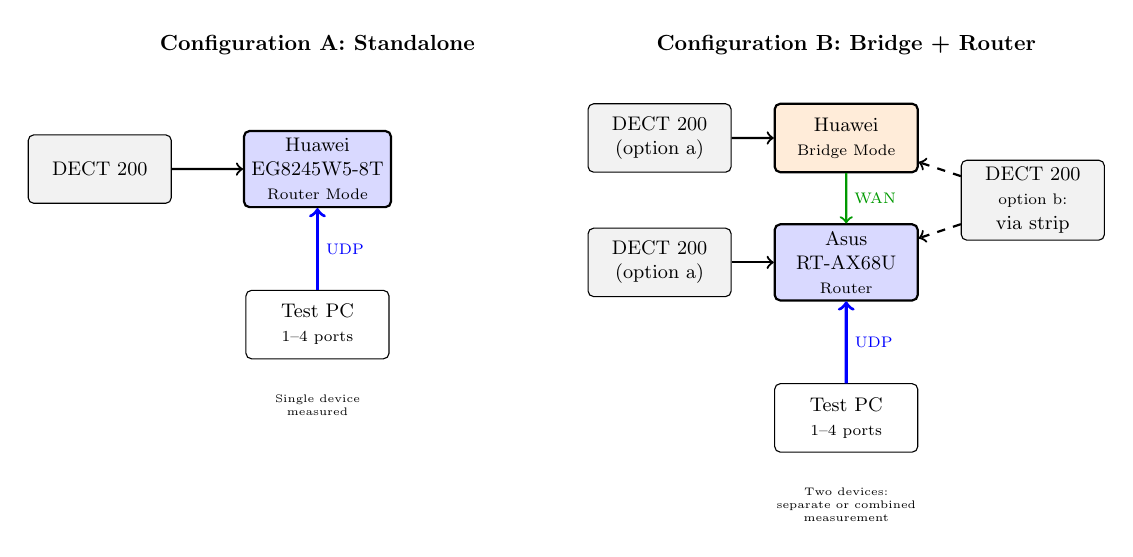
\begin{tikzpicture}[scale=0.79, transform shape,
        box/.style={rectangle, draw, minimum width=2.3cm, minimum height=1.1cm, text centered, font=\small, align=center, rounded corners=2pt},
        router/.style={box, fill=blue!15, thick},
        bridge/.style={box, fill=orange!15, thick},
        meter/.style={box, fill=gray!10},
    ]
        % Configuration A - Standalone
        \node[font=\bfseries] at (0, 5) {Configuration A: Standalone};
        \node[router] (huawei_a) at (0, 3) {Huawei\\EG8245W5-8T\\\scriptsize Router Mode};
        \node[box] (pc_a) at (0, 0.5) {Test PC\\\scriptsize 1--4 ports};
        \node[meter] (meter_a) at (-3.5, 3) {DECT~200};
        \draw[->, thick] (meter_a) -- (huawei_a);
        \draw[->, very thick, blue] (pc_a) -- node[right, font=\scriptsize] {UDP} (huawei_a);
        \node[font=\tiny, anchor=north, align=center] at (0, -0.5) {Single device\\measured};
        
        % Configuration B - Bridge Mode
        \node[font=\bfseries] at (8.5, 5) {Configuration B: Bridge + Router};
        \node[bridge] (huawei_b) at (8.5, 3.5) {Huawei\\\scriptsize Bridge Mode};
        \node[router] (asus_b) at (8.5, 1.5) {Asus\\RT-AX68U\\\scriptsize Router};
        \node[box] (pc_b) at (8.5, -1) {Test PC\\\scriptsize 1--4 ports};
        \node[meter] (meter_b1) at (5.5, 3.5) {DECT~200\\(option a)};
        \node[meter] (meter_b2) at (5.5, 1.5) {DECT~200\\(option a)};
        \node[meter] (meter_b_shared) at (11.5, 2.5) {DECT~200\\\scriptsize option b:\\via strip};
        
        \draw[->, thick] (meter_b1) -- (huawei_b);
        \draw[->, thick] (meter_b2) -- (asus_b);
        \draw[->, thick, dashed] (meter_b_shared) -- (huawei_b);
        \draw[->, thick, dashed] (meter_b_shared) -- (asus_b);
        \draw[->, thick, green!60!black] (huawei_b) -- node[right, font=\scriptsize] {WAN} (asus_b);
        \draw[->, very thick, blue] (pc_b) -- node[right, font=\scriptsize] {UDP} (asus_b);
        \node[font=\tiny, anchor=north, align=center] at (8.5, -2) {Two devices:\\separate or combined\\measurement};
    \end{tikzpicture}
    \caption{Test~5 topology comparison. Configuration~A uses the Huawei in full router mode. Configuration~B splits functionality: Huawei in bridge mode (pass-through) with Asus as the primary router. Power can be measured per-device (two DECT~200 plugs) or as a combined system (single plug via power strip).}
    \label{fig:test5_bridge_topology}
\end{figure}

\subsubsection{Test Protocol}
Both configurations are tested with the same incremental port load profile as Test~1 for direct comparability:
\begin{enumerate}
    \item \textbf{Pre-test baseline} (10\,min): Cables connected, no traffic.
    \item \textbf{Load phases} (4$\times$20\,min): Incremental 1--4 port UDP flood.
    \item \textbf{Post-test baseline} (10\,min): Traffic stopped.
\end{enumerate}

\paragraph{Configuration~A:} Standard Test~1 protocol on the Huawei.
A single DECT~200 smart plug measures total Huawei power.

\paragraph{Configuration~B:}
\begin{itemize}
    \item Huawei set to bridge mode via its admin interface (disables NAT, DHCP, firewall, optionally Wi-Fi).
    \item Asus RT-AX68U configured as the primary router (WAN port connected to Huawei's LAN port).
    \item Test PC connects to the Asus's LAN ports.
    \item \textbf{Power measurement:} Two options depending on available equipment:
    \begin{enumerate}
        \item[(a)] Two DECT~200 plugs (one per device) --- enables separate per-device power attribution.
        \item[(b)] Both devices on a single DECT~200 via a power strip --- measures combined system power directly.
    \end{enumerate}
\end{itemize}

\noindent\textbf{Load generation parameters:} Identical to Test~1 (UDP, 1400\,bytes, 16 workers, 5\,s polling).

\subsubsection{Research Questions Addressed}
\begin{description}
    \item[RQ9 (Fully addressed):] Comparing Configuration~A total power vs.\ Configuration~B total power (Huawei bridge + Asus router) at each load level reveals whether the bridge-mode split is more or less efficient. The per-device breakdown (if two plugs are available) shows how much power the Huawei saves in bridge mode vs.\ how much the Asus adds.
\end{description}
\todo{Run this test and fill in results.}


% ===========================================================================
% Section 5: Results — Incremental Port Load Test
% ===========================================================================
\section{Results: Incremental Port Load Test}
\label{sec:results}

This section presents the results of Test~1 (Section~\ref{sec:test-incremental-port-load}).
We first present per-device power and throughput profiles, then analyze the data in the context of the research questions addressed by this test.

% ---------------------------------------------------------------------------
\subsection{Per-Device Results}
\label{sec:per-device-results}
% ---------------------------------------------------------------------------

% ===== FRITZBOX =====
\subsubsection{Fritzbox 7530}
\label{sec:results-fritzbox}

\begin{figure}[H]
    \centering
    \begin{tikzpicture}
        \begin{axis}[
            width=0.95\linewidth,
            height=7cm,
            xlabel={Elapsed Time (s)},
            ylabel={Power (mW)},
            xmin=0, xmax=6600,
            ymin=4200, ymax=5800,
            grid=major,
            grid style={gray!30},
            legend pos=north west,
            legend style={font=\small},
            title={Fritzbox 7530 --- Power Consumption Over Time},
            % Phase boundary lines
            extra x ticks={600, 1800, 3000, 4200, 5400},
            extra x tick labels={},
            extra x tick style={grid=major, grid style={dashed, red!50, line width=0.8pt}},
        ]
            \addplot[blue, very thin, each nth point=1] table[col sep=comma, x=ElapsedSeconds, y=PowerMW] {data/fritzbox_data.csv};
            \addlegendentry{Power}

            % Phase labels
            \node[font=\tiny, rotate=90, anchor=south] at (axis cs:300,5700) {Idle};
            \node[font=\tiny, rotate=90, anchor=south] at (axis cs:1200,5700) {1 Port};
            \node[font=\tiny, rotate=90, anchor=south] at (axis cs:2400,5700) {2 Ports};
            \node[font=\tiny, rotate=90, anchor=south] at (axis cs:3600,5700) {3 Ports};
            \node[font=\tiny, rotate=90, anchor=south] at (axis cs:4800,5700) {4 Ports};
            \node[font=\tiny, rotate=90, anchor=south] at (axis cs:6000,5700) {Post};

            % Baseline reference
            \draw[dashed, gray, thin] (axis cs:0,4432) -- (axis cs:6600,4432);
        \end{axis}
    \end{tikzpicture}
    \caption{Fritzbox 7530: Power consumption over time. Dashed vertical lines mark phase transitions (600\,s, 1800\,s, 3000\,s, 4200\,s, 5400\,s). Horizontal dashed line indicates idle baseline (4432\,mW).}
    \label{fig:fritzbox_power}
\end{figure}

\begin{figure}[H]
    \centering
    \begin{tikzpicture}
        \begin{axis}[
            width=0.95\linewidth,
            height=7cm,
            xlabel={Elapsed Time (s)},
            ylabel={Throughput (Mbps)},
            xmin=0, xmax=6600,
            ymin=0, ymax=4500,
            grid=major,
            grid style={gray!30},
            legend pos=north west,
            legend style={font=\small},
            title={Fritzbox 7530 --- Aggregate Throughput Over Time},
            extra x ticks={600, 1800, 3000, 4200, 5400},
            extra x tick labels={},
            extra x tick style={grid=major, grid style={dashed, red!50, line width=0.8pt}},
        ]
            \addplot[teal, very thin, each nth point=1] table[col sep=comma, x=ElapsedSeconds, y=ThroughputTotalMbps] {data/fritzbox_data.csv};
            \addlegendentry{Throughput}
        \end{axis}
    \end{tikzpicture}
    \caption{Fritzbox 7530: Aggregate throughput. Note the significant throughput spikes at phase transitions and the decline in total throughput at 3--4~ports due to CPU saturation.}
    \label{fig:fritzbox_throughput}
\end{figure}

The Fritzbox~7530 showed a clear CPU bottleneck effect: total throughput actually \emph{decreased} when moving from 2 to 3 and 4~ports (from $\sim$2483\,Mbps to $\sim$1827\,Mbps aggregate), while power remained relatively flat around 5000--5130\,mW.
The idle baseline averaged 4432\,mW ($\pm$19\,mW).
The post-test baseline was notably higher and more variable (4531\,mW $\pm$223\,mW), suggesting thermal effects or delayed power state recovery.

% ===== HUAWEI =====
\subsubsection{Huawei EchoLife EG8245W5-8T}
\label{sec:results-huawei}

\begin{figure}[H]
    \centering
    \begin{tikzpicture}
        \begin{axis}[
            width=0.95\linewidth,
            height=7cm,
            xlabel={Elapsed Time (s)},
            ylabel={Power (mW)},
            xmin=0, xmax=6600,
            ymin=8600, ymax=9800,
            grid=major,
            grid style={gray!30},
            legend pos=north west,
            legend style={font=\small},
            title={Huawei EG8245W5-8T --- Power Consumption Over Time},
            extra x ticks={600, 1800, 3000, 4200, 5400},
            extra x tick labels={},
            extra x tick style={grid=major, grid style={dashed, red!50, line width=0.8pt}},
        ]
            \addplot[blue, very thin, each nth point=1] table[col sep=comma, x=ElapsedSeconds, y=PowerMW] {data/huawei_data.csv};
            \addlegendentry{Power}
            \draw[dashed, gray, thin] (axis cs:0,8962) -- (axis cs:6600,8962);

            \node[font=\tiny, rotate=90, anchor=south] at (axis cs:300,9700) {Idle};
            \node[font=\tiny, rotate=90, anchor=south] at (axis cs:1200,9700) {1 Port};
            \node[font=\tiny, rotate=90, anchor=south] at (axis cs:2400,9700) {2 Ports};
            \node[font=\tiny, rotate=90, anchor=south] at (axis cs:3600,9700) {3 Ports};
            \node[font=\tiny, rotate=90, anchor=south] at (axis cs:4800,9700) {4 Ports};
            \node[font=\tiny, rotate=90, anchor=south] at (axis cs:6000,9700) {Post};
        \end{axis}
    \end{tikzpicture}
    \caption{Huawei EG8245W5-8T: Power consumption over time. The power profile is very flat, with only $\sim$550\,mW total increase from idle to 4-port full load.}
    \label{fig:huawei_power}
\end{figure}

The Huawei showed the most efficient scaling behavior.
Idle power averaged 8962\,mW, rising monotonically to 9510\,mW under full 4-port load---an increase of only 548\,mW (+6.1\%) while achieving $\sim$3815\,Mbps aggregate throughput (near the theoretical 4$\times$1\,Gbps maximum).
The post-test baseline returned cleanly to 8986\,mW, within 24\,mW of the pre-test value.

% ===== ASUS =====
\subsubsection{Asus RT-AX68U}
\label{sec:results-asus}

\begin{figure}[H]
    \centering
    \begin{tikzpicture}
        \begin{axis}[
            width=0.95\linewidth,
            height=7cm,
            xlabel={Elapsed Time (s)},
            ylabel={Power (mW)},
            xmin=0, xmax=6600,
            ymin=7900, ymax=9500,
            grid=major,
            grid style={gray!30},
            legend pos=north west,
            legend style={font=\small},
            title={Asus RT-AX68U --- Power Consumption Over Time},
            extra x ticks={600, 1800, 3000, 4200, 5400},
            extra x tick labels={},
            extra x tick style={grid=major, grid style={dashed, red!50, line width=0.8pt}},
        ]
            \addplot[blue, very thin, each nth point=1] table[col sep=comma, x=ElapsedSeconds, y=PowerMW] {data/asus_data.csv};
            \addlegendentry{Power}
            \draw[dashed, gray, thin] (axis cs:0,8226) -- (axis cs:6600,8226);

            \node[font=\tiny, rotate=90, anchor=south] at (axis cs:300,9400) {Idle};
            \node[font=\tiny, rotate=90, anchor=south] at (axis cs:1200,9400) {1 Port};
            \node[font=\tiny, rotate=90, anchor=south] at (axis cs:2400,9400) {2 Ports};
            \node[font=\tiny, rotate=90, anchor=south] at (axis cs:3600,9400) {3 Ports};
            \node[font=\tiny, rotate=90, anchor=south] at (axis cs:4800,9400) {4 Ports};
            \node[font=\tiny, rotate=90, anchor=south] at (axis cs:6000,9400) {Post};
        \end{axis}
    \end{tikzpicture}
    \caption{Asus RT-AX68U: Power consumption over time. Shows a clear step-wise increase with each additional loaded port.}
    \label{fig:asus_power}
\end{figure}

The Asus RT-AX68U demonstrated excellent throughput scaling (achieving $\sim$3816\,Mbps at 4~ports) with a moderate power increase from 8226\,mW idle to 8933\,mW at full load (+707\,mW, +8.6\%).
The power increase per additional port was approximately 175\,mW on average.
Post-test recovery was prompt, returning to 8257\,mW ($+$31\,mW from pre-test).

% ===== ALCATEL =====
\subsubsection{Alcatel HH40V}
\label{sec:results-alcatel}

\begin{figure}[H]
    \centering
    \begin{tikzpicture}
        \begin{axis}[
            width=0.95\linewidth,
            height=7cm,
            xlabel={Elapsed Time (s)},
            ylabel={Power (mW)},
            xmin=0, xmax=4200,
            ymin=1600, ymax=2300,
            grid=major,
            grid style={gray!30},
            legend pos=north west,
            legend style={font=\small},
            title={Alcatel HH40V --- Power Consumption Over Time},
            extra x ticks={600, 1800, 3000},
            extra x tick labels={},
            extra x tick style={grid=major, grid style={dashed, red!50, line width=0.8pt}},
        ]
            \addplot[blue, very thin, each nth point=1] table[col sep=comma, x=ElapsedSeconds, y=PowerMW] {data/alcatel_data.csv};
            \addlegendentry{Power}
            \draw[dashed, gray, thin] (axis cs:0,1854) -- (axis cs:4200,1854);

            \node[font=\tiny, rotate=90, anchor=south] at (axis cs:300,2250) {Idle};
            \node[font=\tiny, rotate=90, anchor=south] at (axis cs:1200,2250) {1 Port};
            \node[font=\tiny, rotate=90, anchor=south] at (axis cs:2400,2250) {2 Ports};
            \node[font=\tiny, rotate=90, anchor=south] at (axis cs:3600,2250) {Post};
        \end{axis}
    \end{tikzpicture}
    \caption{Alcatel HH40V: Power consumption over time. Only 2 ports available (100\,Mbps each). Despite low absolute power, the relative increase per port is significant.}
    \label{fig:alcatel_power}
\end{figure}

The Alcatel~HH40V, with only two 100\,Mbps ports, showed the lowest absolute power consumption (idle: 1854\,mW).
Under full 2-port load, power rose to 2076\,mW ($+$222\,mW, $+$12.0\%).
Throughput reached $\sim$257\,Mbps total across both ports (close to the theoretical 200\,Mbps maximum; the slightly higher measured value likely includes transient measurement artifacts from the 5-second polling window).

% ---------------------------------------------------------------------------
\subsection{Cross-Device Comparison}
\label{sec:cross-device-comparison}
% ---------------------------------------------------------------------------

% ===== RQ1: Power vs Port Count =====
\subsubsection{RQ1: Power Consumption vs.\ Number of Active Ports}
\label{sec:rq1-results}

Table~\ref{tab:power-per-phase} summarizes the average power consumption during each load phase for all four devices.

\begin{table}[H]
    \centering
    \caption{Average power consumption (mW) by load phase for each device. $\Delta$ columns show the increase relative to the idle baseline.}
    \label{tab:power-per-phase}
    \footnotesize
    \begin{tabular}{l r r r r r r r r}
        \toprule
        \textbf{Device} & \textbf{Idle} & \textbf{1\,Pt} & $\Delta$ & \textbf{2\,Pt} & $\Delta$ & \textbf{3\,Pt} & \textbf{4\,Pt} & $\Delta_{\text{max}}$ \\
        \midrule
        Fritzbox 7530   & 4432 & 4800 & +368  & 5055 & +623  & 5040 & 5132 & +700 (+15.8\%) \\
        Huawei EG8245W5 & 8962 & 9231 & +269  & 9409 & +447  & 9494 & 9510 & +548 (+6.1\%) \\
        Asus RT-AX68U   & 8226 & 8726 & +500  & 8806 & +580  & 8852 & 8933 & +707 (+8.6\%) \\
        Alcatel HH40V   & 1854 & 1977 & +123  & 2076 & +222  & ---  & ---  & +222 (+12.0\%) \\
        \bottomrule
    \end{tabular}
\end{table}

\begin{figure}[H]
    \centering
    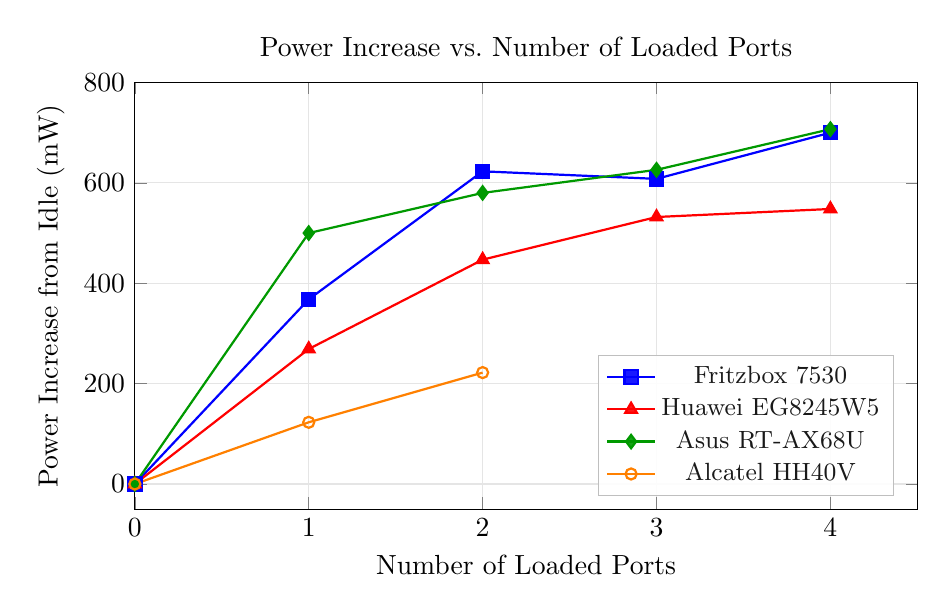
\begin{tikzpicture}
        \begin{axis}[
            width=0.95\linewidth,
            height=7cm,
            xlabel={Number of Loaded Ports},
            ylabel={Power Increase from Idle (mW)},
            xmin=0, xmax=4.5,
            ymin=-50, ymax=800,
            xtick={0,1,2,3,4},
            grid=major,
            grid style={gray!20},
            legend pos=south east,
            legend style={font=\small, fill=white, fill opacity=0.9, draw=gray!50},
            title={Power Increase vs.\ Number of Loaded Ports},
            mark options={scale=1.2},
        ]
            % Fritzbox: 0, +368, +623, +608, +700
            \addplot[blue, thick, mark=square*] coordinates {
                (0,0) (1,368) (2,623) (3,608) (4,700)
            };
            \addlegendentry{Fritzbox 7530}

            % Huawei: 0, +269, +447, +532, +548
            \addplot[red, thick, mark=triangle*] coordinates {
                (0,0) (1,269) (2,447) (3,532) (4,548)
            };
            \addlegendentry{Huawei EG8245W5}

            % Asus: 0, +500, +580, +626, +707
            \addplot[green!60!black, thick, mark=diamond*] coordinates {
                (0,0) (1,500) (2,580) (3,626) (4,707)
            };
            \addlegendentry{Asus RT-AX68U}

            % Alcatel: 0, +123, +222 (only 2 ports)
            \addplot[orange, thick, mark=o, mark options={solid, fill=orange}] coordinates {
                (0,0) (1,123) (2,222)
            };
            \addlegendentry{Alcatel HH40V}
        \end{axis}
    \end{tikzpicture}
    \caption{Power increase above idle baseline as a function of loaded port count. By plotting the delta from each device's idle power, all four devices become directly comparable regardless of their absolute power level. Note the Fritzbox's dip at 3~ports (CPU saturation reduces throughput and thus power). The Alcatel has only 2 ports.}
    \label{fig:power_delta_comparison}
\end{figure}

\paragraph{Key Findings for RQ1:}
\begin{itemize}
    \item All devices show a measurable power increase when ports are loaded, ranging from +222\,mW (Alcatel, 2~ports) to +707\,mW (Asus, 4~ports).
    \item The \textbf{Fritzbox~7530} exhibits a non-monotonic power profile: power peaks at 2~ports (5055\,mW) and then \emph{decreases} at 3~ports (5040\,mW). This is due to CPU saturation---the device cannot sustain full throughput on 3+ ports, so it does less total work and consumes slightly less power. This is a noteworthy finding: under CPU-bound conditions, adding more loaded ports can actually \emph{reduce} total power consumption because the bottleneck shifts from the PHY/switching fabric to the CPU.
    \item The \textbf{Huawei} and \textbf{Asus} devices show monotonically increasing power with near-linear throughput scaling, indicating their CPUs are not the bottleneck at 4$\times$1\,Gbps.
    \item The per-port power increment is small relative to idle power: approximately 30--175\,mW per additional loaded port, depending on the device.
\end{itemize}

% ===== RQ4 (Partial): Idle Power Suitability =====
\subsubsection{RQ4 (Partial): Idle Power and Continuous Operation Suitability}
\label{sec:rq4-results}

Table~\ref{tab:idle-power} presents the idle power measurements and estimated annual energy costs.

\begin{table}[H]
    \centering
    \caption{Idle power consumption ranking and estimated annual energy cost (at €0.25/kWh).}
    \label{tab:idle-power}
    \footnotesize
    \begin{tabular}{l r r r}
        \toprule
        \textbf{Device} & \textbf{Idle Power (W)} & \textbf{Annual Energy (kWh)} & \textbf{Annual Cost (€)} \\
        \midrule
        Alcatel HH40V       & 1.85 &  16.2 &  4.06 \\
        Fritzbox 7530       & 4.43 &  38.8 &  9.70 \\
        Asus RT-AX68U       & 8.23 &  72.1 & 18.01 \\
        Huawei EG8245W5-8T  & 8.96 &  78.5 & 19.63 \\
        \bottomrule
    \end{tabular}
\end{table}

\begin{figure}[H]
    \centering
    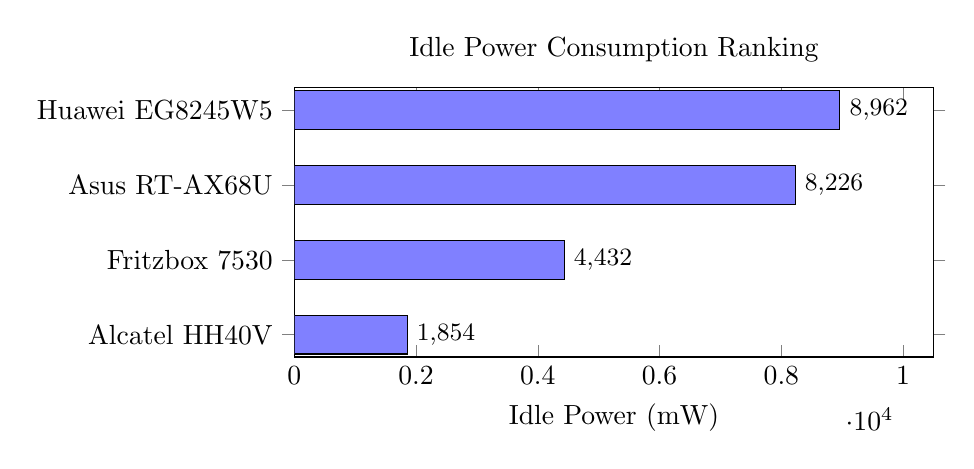
\begin{tikzpicture}
        \begin{axis}[
            xbar,
            width=0.80\textwidth,
            height=5cm,
            xlabel={Idle Power (mW)},
            symbolic y coords={Alcatel HH40V, Fritzbox 7530, Asus RT-AX68U, Huawei EG8245W5},
            ytick=data,
            nodes near coords,
            nodes near coords style={font=\small},
            xmin=0, xmax=10500,
            bar width=14pt,
            title={Idle Power Consumption Ranking},
        ]
            \addplot[fill=blue!50] coordinates {(1854,Alcatel HH40V) (4432,Fritzbox 7530) (8226,Asus RT-AX68U) (8962,Huawei EG8245W5)};
        \end{axis}
    \end{tikzpicture}
    \caption{Idle power ranking. The Alcatel draws less than half the power of the Fritzbox and less than a quarter of the Asus/Huawei devices.}
    \label{fig:idle_power_ranking}
\end{figure}

\paragraph{Key Findings for RQ4 (Partial):}
\begin{itemize}
    \item There is a 4.8$\times$ difference in idle power between the most efficient (Alcatel: 1.85\,W) and least efficient (Huawei: 8.96\,W) device.
    \item Annual idle energy costs range from €4 to nearly €20---a €16 difference that becomes significant in deployments with many access points.
    \item All four devices exceed the typical 2\,W standby threshold discussed in energy efficiency regulations, though the Alcatel is close. However, these are ``cables connected, idle'' measurements, not true standby (which would require disconnecting all Ethernet links and disabling Wi-Fi).
    \item \textbf{Limitation:} These are 10-minute idle measurements. A full 24-hour measurement (as planned for the complete RQ4 analysis) would capture any periodic background activity (firmware updates, Wi-Fi beaconing, DHCP renewal, etc.).
\end{itemize}

% ===== RQ8 (Partial): Rated vs Real Max =====
\subsubsection{RQ8 (Partial): Rated vs.\ Observed Maximum Power}
\label{sec:rq8-results}

Table~\ref{tab:rated-vs-real} compares the manufacturer's rated maximum power with the maximum power observed during the test.

\begin{table}[H]
    \centering
    \caption{Rated maximum vs.\ observed maximum power under full Ethernet load. The ``Utilization'' column indicates what fraction of the rated maximum was reached.}
    \label{tab:rated-vs-real}
    \footnotesize
    \begin{tabular}{l r r r r}
        \toprule
        \textbf{Device} & \textbf{Rated (W)} & \textbf{Observed (W)} & \textbf{Utilization} & \textbf{Headroom (W)} \\
        \midrule
        Fritzbox 7530       & 18 & 5.65 & 31.4\% & 12.35 \\
        Huawei EG8245W5-8T  & 24 & 9.58 & 39.9\% & 14.42 \\
        Asus RT-AX68U       & 33 & 9.22 & 27.9\% & 23.78 \\
        Alcatel HH40V       & 10 & 2.14 & 21.4\% & 7.86 \\
        \bottomrule
    \end{tabular}
\end{table}

\paragraph{Key Findings for RQ8 (Partial):}
\begin{itemize}
    \item None of the tested devices came close to their rated maximum power. The highest utilization was the Huawei at 39.9\% of its 24\,W rating.
    \item The rated maximum appears to account for \emph{all} subsystems operating simultaneously (Ethernet at full load \emph{plus} Wi-Fi radios active with clients \emph{plus} USB peripherals). Since this test only exercised Ethernet ports, significant power headroom remains.
    \item The \textbf{Asus RT-AX68U} has the largest gap: its 33\,W rating vs.\ 9.22\,W observed suggests that the Wi-Fi 6 radios (especially the 5\,GHz radio) likely account for a substantial portion of the rated maximum.
    \item \textbf{Limitation:} To fully answer RQ8, future tests should activate all subsystems simultaneously (Ethernet + Wi-Fi + USB) and attempt to reach the rated maximum.
\end{itemize}

% ---------------------------------------------------------------------------
\subsection{Measurement Considerations}
\label{sec:measurement-considerations}
% ---------------------------------------------------------------------------

Several factors should be considered when interpreting these results:

\begin{enumerate}
    \item \textbf{Power meter resolution:} The DECT~200 reports power in discrete steps of approximately 70\,mW. For devices where the load-induced power increase is small (e.g., Huawei: $\sim$550\,mW over 4~ports), the per-port incremental power ($\sim$137\,mW) is only about 2 discrete steps, limiting measurement precision for fine-grained per-port analysis.
    \item \textbf{CPU-targeted traffic:} All traffic was directed at the device's own IP, engaging the CPU stack rather than the hardware switching fabric. A Layer~2 forwarding test (e.g., port A$\rightarrow$B loopback) would likely show different power characteristics.
    \item \textbf{No zero-cable baseline:} The pre-test baseline had all cables physically connected (link up, no traffic). The power cost of merely maintaining a GbE link (PHY active, auto-negotiation) vs.\ having no cable connected was not isolated.
    \item \textbf{Throughput anomalies:} Some data points show transient throughput spikes (especially the Fritzbox and Alcatel) that exceed steady-state values. These are measurement artifacts caused by buffered packet bursts aligning with the 5-second polling window.
\end{enumerate}

% ---------------------------------------------------------------------------
\subsection{Summary of Findings}
\label{sec:results-summary}
% ---------------------------------------------------------------------------

Table~\ref{tab:results-summary} provides a comprehensive comparison of all key metrics across the four devices.

\begin{table}[H]
    \centering
    \caption{Comprehensive summary of Test~1 results across all four devices.}
    \label{tab:results-summary}
    \small
    \begin{tabular}{l r r r r}
        \toprule
        \textbf{Metric} & \textbf{Fritzbox} & \textbf{Huawei} & \textbf{Asus} & \textbf{Alcatel} \\
        \midrule
        Idle Power (mW)              & 4432  & 8962  & 8226  & 1854 \\
        Max Load Power (mW)          & 5132  & 9510  & 8933  & 2076 \\
        Power Increase (mW)          & +700  & +548  & +707  & +222 \\
        Power Increase (\%)          & 15.8  & 6.1   & 8.6   & 12.0 \\
        Max Throughput (Mbps)        & 2483  & 3815  & 3816  & 257 \\
        Theoretical Max (Mbps)       & 4000  & 4000  & 4000  & 200 \\
        Throughput Achieved (\%)     & 62.1  & 95.4  & 95.4  & 128.5\textsuperscript{*} \\
        Peak Efficiency (Mbps/W)     & 491   & 401   & 427   & 124 \\
        Rated Max (W)                & 18    & 24    & 33    & 10 \\
        Rated Utilization (\%)       & 31.4  & 39.9  & 27.9  & 21.4 \\
        \bottomrule
        \multicolumn{5}{l}{\textsuperscript{*}\scriptsize Measurement artifact: 5-second polling window captures burst averages above 200\,Mbps.} \\
    \end{tabular}
\end{table}

This concludes the analysis of Test~1. The remaining research questions (RQ2, RQ3, RQ5--RQ7, RQ9) require additional test setups as described in Section~\ref{sec:test-setups}.
\todo{Add results for Tests 2--5 as they are completed.}


        %% 
%%%%%%%%%%%%%%%%%%%%%%%%%%%%%%%%%%%%%%%%%%%%%%%%%%%%%%%%%%%%%%%%%%%%%%%%%%%%%%%%

%%%%%%%%%%%%%%%%%%%%%%%%%%%%%%%%%%%%%%%%%%%%%%%%%%%%%%%%%%%%%%%%%%%%%%%%%%%%%%%%
%% 
%% Print the bibliography
%% 
%% (Optionally) let the bibliography start on a new odd page (odd is only relevant in twoside layout)
%\cleardoubleoddpage
\printbibliography
%% 
%%%%%%%%%%%%%%%%%%%%%%%%%%%%%%%%%%%%%%%%%%%%%%%%%%%%%%%%%%%%%%%%%%%%%%%%%%%%%%%%
\newpage
%% Begin with the appendix part (all further sections will be appendices)
\appendix

%%%%%%%%%%%%%%%%%%%%%%%%%%%%%%%%%%%%%%%%%%%%%%%%%%%%%%%%%%%%%%%%%%%%%%%%%%%%%%%%
%% 
%% Add your appendix sections ...
%% 

%% Make sure to start the appendix on a new odd page (odd is only relevant in twoside layout)
%\cleardoubleoddpage
\section{An Appendix}
\label{app:an-appendix}

Fritzbox Web UI password: Ins2025 Wi-Fi password: default (printed on router)

%% 
%%%%%%%%%%%%%%%%%%%%%%%%%%%%%%%%%%%%%%%%%%%%%%%%%%%%%%%%%%%%%%%%%%%%%%%%%%%%%%%%

\cleardoubleoddpage

\end{document}
\endinput
